\section{OUR APPROACH}
\label{sec:appr}
%\KZ{In all algorithm listings, specify clearly which parameters are
%input and which are output. Go thru the algos carefully to make sure that
%there's no errors. You can check out the semantics-similarity folder under
%papers in the svn repo to see how that paper writes algo with input
%and output. Notice that function should have a return statement and
%procedure has none.}

In this section, we propose a novel watermarking approach, 
which can effectively survive ``massive crop'' and ``merge'' attacks.
%by accurately identifying the regions that might have been watermarked. 
Our watermarking method %uses a small amount of spatial information of the original
%map as the secret key and 
inserts negligible watermarks (one-bit only)
to locations which are determined by a spatial partitioning algorithm.
Then during detection time, the same spatial partitioning algorithm is used
with the help of a secret key, which ensures that the resulting segmentation of
the space and the input map is almost identical to that of the watermarked map,
even though no original map is available.
%Then we introduce our approach in 
%details and finally preform some reliability analysis. 
%We can identify two main parts in designing a digital road map watermarking algorithm, 
%Insertion and Detection. In the first part, a strategy has to be designed to insert 
%some secret watermarks into original digital road maps. In this part, the workflow can 
%also be divided into two steps. Firstly, a small secret subset in which all 
%data points will be watermarked is selected from the whole digital map dataset. 
%Secondly, the selected small dataset is inserted with secret watermarks. 
%In the second part, according to the strategy of insertion, watermarks hidden in the 
%data set are detected and extracted from  the watermarked data set. 
In the following, we first introduce the secret keys used in this framework,
then present the space partitioning algorithm, watermark insertion and detection
algorithms, before giving analysis of the algorithms. All symbols used in the algorithms
are summarized in \tabref{tab:para}.

\begin{table}[th]
\centering
\caption{All Symbols Used in Algorithms}
\label{tab:para}
\begin{tabular}{|c|c||c|c|} 
\hline
\bf Symbol & \bf Definition & \bf Symbol & \bf Definition \\\hline \hline
$G$ & master grid & $PO$ & sub-region list \\\hline
$M$ & original data-set & $T$ & MQtree \\\hline
$\R$& partitioned region & $l$& secret square size \\\hline
$\theta$ & road length threshold & $k$& secret hash key\\\hline
\end{tabular}
\end{table}

\subsection{Secret Keys}
The secret keys, often randomly generated, are used to decide where to insert the 
watermarks. In the proposed algorithm, we use three secret keys: 
a master grid, a secret minimum bounding rectangle (MBR) and
a secret square size. 
%We explain these keys one by one next. 

%\subsubsection{Master Gird}
The {\em master grid} $G$ is a secret coordinate system which is only known
to the map producer. The grid has an origin which is certain position on earth
with precise latitude and longitude, and it has a step size which defines
the granularity of the grid (see \figref{fig:grid}):
\[G=\{Origin(x_0, y_0), Step\}\]

%\subsubsection{Secret MBR}
%This partitioning need to be kept in secret so that the attackers will not know which 
%region will a data point locate. In our algorithm, we partition the space according to 
%Quadtree, so what we need to keep in secret is the initial Minimum Boarder Rectangle(MBR) of the map. 
%We create a grid frame randomly, impose secret grid frame on the map and select 
%smallest regions(MBR) from grid frame that completely cover the whole map.
Given an original map to watermark, it can be laid out on the master grid, 
according to the coordinates of the vertices in the map. 
The {\em secret MBR} is then the smallest
rectangle which coincides with the grid lines and completely 
encloses the whole map. The red rectangle in \figref{fig:grid} 
is one such secret MBR of the blue road map. 
In our algorithm, we partition the space according to a modified Quadtree. 
The MBR of the map serves as an initial of the partition process,
which will improve the robustness of our algorithm.  
%This MBR is unique per map and it stores only
%minimal information about the position of the map in the master grid.

\begin{figure}[th]
\centering
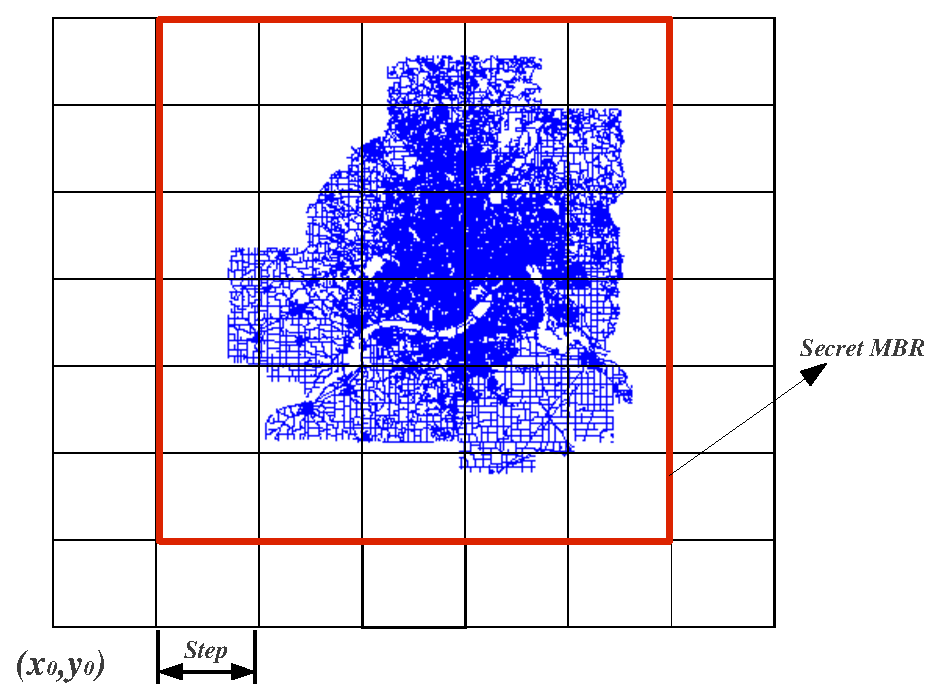
\epsfig{file=images/SecretGrid.eps,width=0.8\columnwidth}
\caption{Master Grid and MBR}
\label{fig:grid}
\end{figure}

%\subsubsection{Secret Square Size}
The {\em secret square size} is an integer number $l$ that determines the size of a square box that we
used to select a small neighborhood of road segments from which to compute the watermarks.
More details of the use of $l$ will be presented in \secref{sec:insert}. 
%In insertion and detection parts of our algorithm, another two secret keys
%are applied. To determine the position to insert watermark of the selected points,
%we use a square centered at the selected data point with a secret side length to 
%choose the neighbourhood road segments. This process could be illustrated by Figure
%\ref{fig:13}. When hashing to get the target position, a secret random table is also used.

\subsection{Space Partitioning Algorithm}

\algoref{Partition} is used in both insertion and detection 
of the watermarks. 
It recursively partitions the space bounded by the secret MBR for a map
into small regions using a modified quad-tree
structure (known as MQtree) according to the 
density of the roads. Each node in MQtree represents a sub-region of the map.
A leaf node represents a region in which the total length of road segments
within is between $\theta$ and $4\theta$ meters. %, where $\theta$ is a parameter of the algorithm. 
\figref{fig:mqtree} illustrate a MQtree created from partitioning an MBR
shown in \figref{fig:par}. 
%The details are listed in \algoref{Partition}.

%Leaf nodes represent those subregions that is partitioned in the deepest level. 
%Non-leaf nodes represent the areas consisting of all subareas represented by their children. In Figure \ref{fig:quadtree}, subregion one is partitioned two times, since its road density is greater. The second subregion is not partitioned since the road in it is more sparce.

\begin{figure}[th]
\centering
\subfigure[\scriptsize Map]{
  \label{fig:par}
  \epsfig{file=images/partition.eps,width=0.35\columnwidth}
}
\subfigure[\scriptsize MQtree]{
  \label{fig:mqtree}
  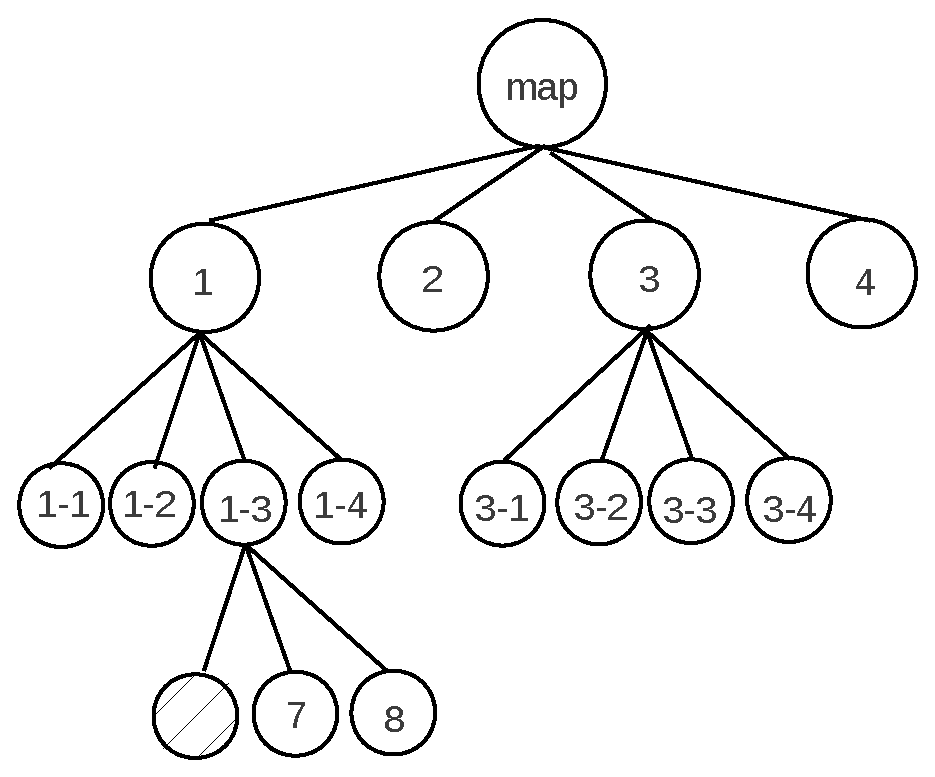
\epsfig{file=images/MQtree.eps,width=0.45\columnwidth}
}
\caption{MQtree}
\label{fig:quadtree}
\end{figure}

In \algoref{Partition}, the secret MBR is generated from the master grid(see Figure \ref{fig:grid}). 
Then the map area is partitioned iteratively according to the density of roads 
such that finally the total road length included in every subregion has more 
than m meters and less than $4 * \theta$ meters. Finally, we output all of 
these subregions. Here we modify Quadtree by merging one subregion with less roads 
with its smallest neighbor when the road length of it is less than $\theta$.
%The partition algorithm must create roughly the same kind of segmentation
%result on the same map, with or without watermarks, before or after attacks.
Road length of an area cannot be changed arbitrarily
due to the constraints of perception tolerance which must be observed by both
the watermark producer and the attacker. No matter a watermarked map is cropped 
or merged with other parts from different maps, this method still produces 
almost the identical partition results for the watermarked part. 



\begin{algorithm}[th]
\caption{Partition}
\label{Partition}
\begin{algorithmic}[1]
\Require $G$, $M$, $T$, $\theta$
\Ensure $PO$, $T$
\Function{PARTITION}{$G,~M,~T,~\theta$}
\State $L|PO|T\leftarrow$new queue$|$new list$|MBR(G,~M)$
%\State $\leftarrow$new list
%\State $\leftarrow MBR(G,~M)$
\State $L.Push(T)$
\While{$L$ is not empty}
\State partition region $\R \leftarrow L.pop$ into ${\R}_{i}$, $i\in \left\{1,2,3,4\right\}$
\For{each ${\R}_{i}$}
\If{road length in ${\R}_{i} < \theta$}
\State merge ${\R}_{i}$ with its smaller neighbor
\ElsIf{road length in ${\R}_{i} > 4 \theta$}
\State $\R.children_i \leftarrow {\R}_{i}$ 
\State  $L.push(\R.children_i)$
\Else{}
\State $\R.children_i \leftarrow {\R}_{i}$
\State insert ${\R}_{i}$ to $PO$
\EndIf
\EndFor
\EndWhile\\
\Return $PO$
\EndFunction
\end{algorithmic}
\end{algorithm}

\subsection{Watermark Insertion Algorithm}
\label{sec:insert}
\begin{figure}[bh]
\centering
\epsfig{file=images/insertion.eps,width=0.4\columnwidth}
\caption{Insertion Strategy %\KZ{I think in this fig you want draw a 
%dashed line circle
%centered at the center of the square box and this circle touches on P(x, y)
%to show how to find P(x, y)}
}
\label{fig:insert}
\end{figure} 

\algoref{algo:Insertion} first generates a set of sub-regions by partitioning. 
Then it inserts one watermark into each sub-region at the leaf nodes of the 
MQtree. The watermark is inserted into a road vertex $P(x, y)$ which is
closest to the center of the sub-region (marked by the black box in 
\figref{fig:insert}). To compute the exact watermark to be inserted, the algorithm
then draw a square box of size $l$ (the other secret key) centered at
$P(x, y)$ (the red box in \figref{fig:insert}). Let $sl$ be the length of road
segments that intersects the square box, and let $j$ be a value hashed from
$sl$. We then set the $j^{th}$ least significant bit in $x$ coordinate of $P$ 
to ``1''. The hash function in this algorithm must 
guarantee to hash to the same value before and after watermarking. 
Even if the watermarked map is attacked 
(i.e., some end points of those segments intersecting $Q$ are altered),
the hash function must still hash to the same $j$. To this end, we design this 
function with a tolerance to possible distortions. Assuming that the 
biggest possible distortion of a single end point is the change of
$J_{max}$ least significant bits of the coordinates, then
\begin{eqnarray*}
j&=&Hash(Trans(sl),k) \\
&\rm{where} & Trans(x)= x \land \underbrace {11\ldots1\overbrace {00\ldots0}^{J_{max}} }_{bit\_length(x)} 
\end{eqnarray*}
%\KZ{This hash function is critical. We need to show what exactly is this
%function. How can we make sure that it has the necessary tolerance to
%defeat possible distortion?} 

%
%To find the right vertex, we use a square of size $l$ centered at the selected data 
%point $P$ with a secret side length to choose the neighbourhood 
%road segments which interest the very square (see Figure \ref{fig:insert}). 
%In Algorithm \ref{Insertion}, we 
%Then data points closest to the center of subregions are selected to watermark. 
%We watermark the selected data points according to their neighbors in space. 
%Specifically, 
%Then we can summarize the total number of these segments and hash 
%it with a secret random table to a certain least significant bit (LSB) position. 
%Then we set the corresponding LSB value for the selected data point to be ``1''.

\begin{algorithm}[th]
\caption{Insert Watermark into Map}
\label{algo:Insertion}
\begin{algorithmic}[1]
\Require $G$, $M$, $l$, $k$, $\theta$
\Ensure $M$
\Procedure{INSERTION}{$M,~G,~l,~k,~\theta$}
\State $PO\leftarrow$ PARTITION( $G,~M,~NULL,~\theta$ )
\For{each region ${\R}_{i} \in PO$}
\If {road length in ${\R}_{i}>\theta$}
\State $P\leftarrow$ point closest to ${\R}_{i}.center$
\State draw a square $Q$ of side length $l$ centered at $P$
\State $sl \leftarrow$ length of line segments intersecting $Q$
\State j $\leftarrow$ Hash( $k,sl$ )
\State $j^{th}$ LSB of $P.x \leftarrow$ 1
\EndIf
\EndFor
\EndProcedure
\end{algorithmic}
\end{algorithm}

\subsection{Watermark Detection Algorithm}

In \algoref{algo:Detection}, we partition the map %into smallest possible subregions
using the same strategy as insertion. Then we select the data points closest
to the center of the regions to detect whether the watermark exists there.
Each sub-region which is detected to contain a watermark casts a vote
which collectively contributes to the final decision of whether a larger
area is watermarked as a whole.
%In \algoref{algo:Detection}, we partition the map that may have been 
%attacked and select the data points to detect. Then we calculate% the total 
%%number of neighbor road segments and compute 
%the watermarked bit location in the same way as in the insertion algorithm. 
%While selecting points, we construct the MQtree which depicts the whole digital map. 
For leaf nodes of the MQtree, if the bit value at the right position is ``1'', we mark 
this sub-region as a ``match''. 
Function STATS($T$) (\algoref{algo:mark}) computes two statistics for
each node of the MQtree: the total number leaf nodes underneath the node ($T$.total)
and the total number of nodes which has been marked as ``match'' ($T$.match).
If the detection confidence $conf(T_i)$ is larger than a threshold $\xi$ for
for any non-leaf node $T_i$, the watermark in the map is successfully identified.
We define the detection confidence of $T$ as
\begin{equation} \label{eqn:conf}
conf (T) =1 - \sum _{ i=n }^N{N \choose i}\left(\frac{1}{2}\right)^{ N-i} 
\left(\frac{1}{2}\right)^i 
\end{equation}
where $N$ is $T$.total and $n$ is $T$.match. 
In our approach, the data points where we select to insert watermark may
already contain ``1'' at the specified bit position. Here we assume uniform
distribution and hence the probability of ``1'' being already present is
1/2.
 
\begin{algorithm}[th]
\caption{Detect Watermark from a Suspicious Map}
\label{algo:Detection}
\begin{algorithmic}[1]
\Require $G$, $M$, $l$, $k$, $\theta$
\Ensure $Yes/No$
\Function{DETECTION}{$M,~G,~l,~k,~\theta$}
\State $T \leftarrow$ new MQtree
\State $PO \leftarrow$ PARTITION( $G,~M,~\&T,~\theta$ )
\For{each region ${\R}_{i} \in PO$}
\If {road length in ${\R}_{i} > \theta$}
\State $P\leftarrow$ point closest to ${\R}_{i}.center$
\State draw a square $Q$ of side length $l$ center at $P$
\State $sl \leftarrow$ length of line segments intersecting $Q$
\State j $\leftarrow$ Hash( $k,sl$ )
\If {$j^{th}$ LSB of $P.x$ is 1}
\State Mark ${\R}_{i}$ as ``match''
\EndIf
\EndIf
\EndFor
\State STATS( $T$ )
\For {each non-leaf node $T_i$ of $T$ in depth-first order}
\If {$conf(T_i) > \xi $}
\Return $Yes$
\EndIf
\EndFor\\
\Return $No$
\EndFunction
\end{algorithmic}
\end{algorithm}

\begin{algorithm}[th]
\caption{Compute Stats For a Given MQtree}
\label{algo:mark}
\begin{algorithmic}[1]
\Statex
\Procedure{STATS}{$T$}
\If{ $T$ is not a leaf node}
\For{each $T_i\in T.children$}
\State STATS(${T}_{i}$)
\State $T$.match$\leftarrow$$T$.match+${T}_{i}$.match
\State $T$.total$\leftarrow$$T$.total+${T}_{i}$.total 
\EndFor
\Else{}
\If{The region of $T$ is ``match''}
\State $T$.match$\leftarrow$1
\Else{}
\State $T$.match$\leftarrow$0
\EndIf
\State $T$.total$\leftarrow$1
\EndIf
\EndProcedure
\end{algorithmic}
\end{algorithm}


%It is obvious that the strategy of detection is similar to that of insertion. 
%We construct a Quadtree and get the knowledge 
%that whether its leaf nodes are `match' or not. 
%Finally, we calculate the ratio of the number of leaf nodes that 
%``match'' to the total number of leaf nodes of this sub-region. 
%If this ratio is greater than a predefined threshold, 
%we conclude that this sub-region of the map contains the watermark.
If the watermarked map is attacked by ``massive crop'' attack, 
the MQtree structure partitioned by detection algorithm is
just a part of the insertion MQtree. 
However, it will be almost the same as the corresponding part of the MQtree 
for the whole map. 
An example of the detection process is illustrated in Figure \ref{fig:detect}. 
Assuming that the shaded parts of \figref{fig:parcrop} is 
cropped from the watermarked map, 
the corresponding MQtree is shown in \figref{fig:mqtreecrop}.

%\begin{figure}[h]
%\centering
%\epsfig{file=detection.eps,width=0.8\columnwidth}
%\caption{Detection Strategy}
%\label{fig:detect}
%\end{figure} 

\begin{figure}[h]
\centering
\subfigure[\scriptsize Map]{
  \label{fig:parcrop}
  \epsfig{file=images/parcrop.eps,width=0.35\columnwidth}
}
\subfigure[\scriptsize MQtree]{
  \label{fig:mqtreecrop}
  \epsfig{file=images/MQtreecrop.eps,width=0.45\columnwidth}
}
\caption{Detection Strategy}
\label{fig:detect}
\end{figure} 

If the watermarked map is attacked by ``Merge Attack'', 
the detection MQtree will be almost the same as the insertion one. 
However, we can find the watermark only in part of the MQtree. 
In this case, the algorithm reports the sub-regions that are watermarked.
We can make a depth-first traversal of the detection MQtree to 
find the largest watermarked region. % (see Algorithm \ref{algo:find}).

%\begin{algorithm}[th]
%\caption{Find the Watermarked Region}
%\label{algo:find}
%\begin{algorithmic}[1]
%\Statex
%\Function{DF\_TRAVERSE}{$T$}
%\If{ $conf(T) < \xi $}
%\State $T$ is $Yes$
%\Else{}
%\For{each ${T}_{i}\in T.children$}
%\State DF\_TRAVERSE(${T}_{i}$)
%\EndFor
%\EndIf\\
%\Return
%\EndFunction
%\Statex
%\end{algorithmic}
%\end{algorithm}

%Computation complexity of Algorithm \ref{algo:Detection} is similar to Algorithm \ref{Insertion}.
  
%\[\T_{detec} = O(|V|\log\LEN).\]



